\documentclass{standalone}
\usepackage{tikz}
\usetikzlibrary{positioning, arrows}

\begin{document}

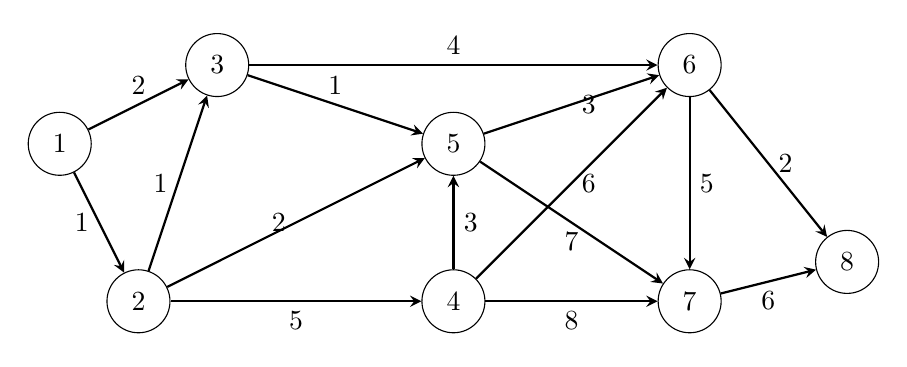
\begin{tikzpicture}[->, >=stealth, node distance=2cm, scale=1, transform shape]

    % Definir nodos con posiciones específicas
    \node[circle, draw, minimum size=0.8cm] (n1) at (0,2) {1};
    \node[circle, draw, minimum size=0.8cm] (n2) at (1,0) {2};
    \node[circle, draw, minimum size=0.8cm] (n3) at (2,3) {3};
    \node[circle, draw, minimum size=0.8cm] (n4) at (5,0) {4};
    \node[circle, draw, minimum size=0.8cm] (n5) at (5,2) {5};
    \node[circle, draw, minimum size=0.8cm] (n6) at (8,3) {6};
    \node[circle, draw, minimum size=0.8cm] (n7) at (8,0) {7};
    \node[circle, draw, minimum size=0.8cm] (n8) at (10,0.5) {8};

    % Definir aristas con pesos
    \path[draw, thick]
    (n1) edge node[above] {2} (n3)
    (n1) edge node[left] {1} (n2)
    (n2) edge node[left] {1} (n3)
    (n2) edge node[below] {5} (n4)
    (n2) edge node[left] {2} (n5)
    (n3) edge node[above] {1} (n5)
    (n3) edge node[above] {4} (n6)
    (n4) edge node[below] {8} (n7)
    (n4) edge node[right] {3} (n5)
    (n4) edge node[right] {6} (n6)
    (n5) edge node[right] {3} (n6)
    (n5) edge node[below] {7} (n7)
    (n6) edge node[right] {2} (n8)
    (n6) edge node[right] {5} (n7)
    (n7) edge node[below] {6} (n8);

\end{tikzpicture}

\end{document}
